\documentclass[11pt, oneside]{article}   	% use "amsart" instead of "article" for AMSLaTeX format
\usepackage{geometry}
\usepackage[linesnumbered]{algorithm2e}
\geometry{letterpaper}
\usepackage{graphicx}
\usepackage{amsmath, amsthm, amssymb}
\usepackage{parskip}
\usepackage{titlesec}
\usepackage{enumerate, float}
\graphicspath{ {images/} }

\newtheorem*{theorem}{Theorem}
\newtheorem*{lem}{Lemma}
%SetFonts
\titleformat{\paragraph}
{\normalfont\normalsize\bfseries}{\theparagraph}{1em}{}
\titlespacing*{\paragraph}
{0pt}{3.25ex plus 1ex minus .2ex}{1.5ex plus .2ex}
\title{CS340 - Registrar's Scheduling Problem}
\author{Yutong Li, Tianming Xu, Jiaping Wang}
\date{\today}							% Activate to display a given date or no date

\begin{document}
\maketitle

\section{Description}
\subsection{Notation}
Let $S$ be the set of students, with $|S|=s$. Each student will have a list of class requests, so let $l_{s_i}$ to represent the $i^{th}$ student's list of class requests. We denote the set of teachers by $P$ and its cardinality by $|P|=p$. Let $C$ be the set of classes, and so we have $|C|=c$ classes. Denote the set of classrooms by $R$, with $|R|=r$, and the set of time slots as $T$, with $|T|=t$. 
\subsection{Algorithm Description}
Given $S, P, C, R, T$, we determine a class schedule with following rule: schedule as many students as possible into each class in decreasing order of the class' popularity, defined by the number of students hoping to take this class. \par 
Start off by sorting the classes in decreasing order of popularity. Sort the classrooms in decreasing order of capacity. \par
Then, we can begin pairing classes with classrooms and time periods. Starting with the most popular class $c_1$, we try scheduling this class in the biggest classroom $r_1$ during its first available time slot $t_1$. Find the teacher $p_1$ who teaches $c_1$. If $p_1$ has no conflict during this time, put the class-room-time combination into the final schedule. Otherwise, add the (room, time) combination as a skipped slot and move on to the next slot. Once this class is scheduled, mark both the teacher and classroom as unavailable during this time period. Repeat this process for the next most popular class in the next time slot, except that if there are previously skipped slots, we try scheduling the class to the skipped slot(s) first. Otherwise, always try scheduling the class in the largest available classroom during its earliest available time slot, checking for conflicts with teacher. Keep doing so until either all classrooms are filled at all times, or all $2m$ classes has been scheduled.\par
After all class time and location are settled for all classes, we proceed to select students for each class in the same order. Starting with the most popular class, as long as there are seats available in the classroom, we randomly select a student from those who signed up for this class. If the student has no conflict at the same time, pair the student with the class. If the student has a conflict, remove him/her from the pool and select another one. Repeat the process until either all seats are filled or all prospective students are considered.
\subsubsection{Haverford Extension}
\underline {\textbf{Additional Constraints}}\par
In order to schedule classes before pre-registration data is available and to more accurately reflect real-life situations at Haverford, we consider the following additional constraints:
\begin{enumerate}
\item There are six core classes for each major. Thus, it is more important to schedule these classes before others.
\item Consider the number of majors and minors in each department to determine the relative popularity of classes.
\item Intro-level classes are likely to have larger size than higher-level classes.
\item Different time slots are allowed to have overlaps.
\item Teachers may have personal time conflicts.
\item Some classes have a lab session, which must be scheduled during a consecutive 3-hour time slot rather than the usual 1-1.5 hour lecture times that are spread out on different days.
\end{enumerate}
%describe our constraints and explain why they are well-reasoned.
\par To determine a popularity rating without preregistration data, we weight the importance of classes based on past enrollment data, the number of majors in its department, class level, and whether a class is core. The number of enrolled students in Spring 2014 is used as a reference value for the expected class size. We also predict popularity based on the number of majors and minors in each department. Classes from popular departments, like Computer Science, are highly demanded each semester. Therefore, making sure these classes are offered is a reasonable move. However, we also want to schedule core classes first because these are the classes students must take to fulfill they graduation requirements. Furthermore, giving priority to core classes when scheduling allows students with less popular majors to finish their majors. Otherwise, if classes in popular departments are always preferred over those in less popular departments, these students might not have enough opportunity to take any class in their major. \par
Besides, we want to consider professors' personal time conflicts to better simulate actual conflict situations. For instance, some professors are fathers/mothers, so probably they won't be able to teach classes between 8:00-10:00 AM or 3:00-5:00 PM because of their children's school schedule. Also, professors who live far from campus and thus require longer commute time would prefer to avoid early morning or late evening classes. \par
 The last additional constraint allows lab session to be associated with lectures, which is very common for natural science classes in our college. This constraint adds the requirement that lectures need to be scheduled during shorter time slots and labs need to be in longer time slots. Furthermore, we also schedule fine arts classes during lab times, since studio work usually require longer class time. However, to simplify the scheduling process, we made the following assumptions:\begin{enumerate}[\label = (1)]
 \item Each class has at most one lab session.
 \item Labs must be scheduled during 3-hour time slots. (No 1-hour labs are considered).
 \item Labs may or may not have the same instructor as the lecture. If a different instructor for a lab course is specified in the Spring 14 data, we schedule it with the lab instructor. Otherwise, we assume it has the same instructor as the lecture.
 \end{enumerate}
\underline {\textbf{Implementation}}\par
%talk about how we implement the constraints
\par From the csv file containing Spring 2014 enrollment data, we can get rooms, time slots, classes, department, class level, and instructor information. Since we don't have the information about whether a class is a core class for some major, we choose the two classes with most enrolled students from each of $100$-, $200$-, and $300$-levels in every department and assign these as core. In addition, every class that has department number WRPR, i.e. is a writing seminar, are also labeled as core, since there must be enough writing seminars for first-years to complete their writing requirement. 
\par For overlapping time slots, we stored each time slot as a tuple with fields, begin time, end time, and days. When the main algorithm checks if a room-time combination is suitable for a particular class, it checks for time overlap with (a) all unavailable time slots of the teacher, and (b) all other classes that have been scheduled in the same room.
\par The popularity of majors is retrieved from the Office of Institutional Research at Haverford College. For each department, we counted the number of majors and minors from Class of 2015 and 2016. This information is stored in an array.
\par For professor's personal conflicts, we randomly assign $0-5$ unavailable time slots for each professor. When trying to add a class to the schedule, the candidate time slot is compared against each one of the professor's unavailable times. If there is an overlap between any pair, we move on to the next slot.
\par Information about labs is also retrieved from the Spring 2014 enrollment data. If a class has $0$ Units Taken, has a section number, and indeed takes longer than 2.5 hours, then we consider it a lab. Each lab course is associated with a lecture and they share the same course number. In the main scheduling algorithm, the set of time slots are separated into two parts: lecture time and lab time, the former usually consists 1 - 1.5 hour in two or three days, and the latter is 3 hours in one sitting. When scheduling classes, we first consider the array of all lectures in sorted order based on their weighted importance. These classes can only be assigned in lecture slots. If a class being scheduled is associated with a lab, we immediately schedule the lab using the first available lab slot after the schedule for lecture is finalized. When choosing students for a given class, if the class has a lab section, we need to check whether the student has conflicts during both lecture and lab times. If the student has been assigned to another class that conflicts with either one, we move on to the next student.
\section{Pseudocode}
\begin{algorithm}[H]
\SetKwBlock{Begin}{Begin}{}
\SetKwFunction{Schedule}{Schedule}
\SetKwProg{Fn}{Function}{}{}
\Fn{\Schedule{S, P, C, R, T}}{
Sort $C$ in decreasing order of popularity.\\
Sort $R$ in decreasing order of capacity.\\
Compute the total number of room-time combinations: $rt$.\\
Let $k=0$ be the class we're scheduling.\\
Let $i=0$ be the first available time slot in the largest available room.\\
Let $skippedSlots$ be a FIFO queue\\
 \While{$i < \min \{c, rt\}$}{
 	\uIf{$skippedSlots$ is empty}{
	        	\While{ $i<rt$ and either teacher or room has a conflict with this slot}{
        			Put $i$ in $skippedSlots$\\
			$i\gets i+1$}
		\If{$i<rt$}{
		Schedule class $k$ in room $\lfloor i/t\rfloor$ at time $(i\mod t)$.}}
        	\Else{
		\While{$skippedSlots$ is not empty }{
	   		Pop $j$ from $skippedSlots$\\
	   		\uIf{ $k$'s teacher has a conflict with the skipped slot}{
	    			Push the slot back to $skippedSlots$}
	   		\Else{
				Schedule class $k$ in room $\lfloor j/t\rfloor$ time $j\mod t$.\\
				\textbf{break}
			}
		}
		\If { $skippedSlots$ is empty and $k$ hasn't been scheduled}{
			Try scheduling $k$ at slot $i$ as in lines 9 - 12, incrementing $i$ if applicable
		}
        	}
	$k\gets k+1$
	}
	\Return $Schedule$
}
\end{algorithm}
\begin{algorithm}[H]
\SetKwBlock{Begin}{Begin}{}
\SetKw{Continue}{continue}
\SetKwFunction{ChooseStudent}{ChooseStudent}
\SetKwProg{Fn}{Function}{}{}
\Fn{\ChooseStudent{Schedule}}{
\For{each scheduled class}{
	\For {each potential students who registered for this class}{
	\If{the classroom is not full}{
		Choose a random student from the list of preregistered students\\
	\uIf{student has another class at this time}{
		\Continue}
	\Else{
		Add this student to the class in schedule}
	}}}
\Return $Schedule$}

\end{algorithm}

\section{Time Analysis}
\subsection{Data Structure}
The class requests of each student can be stored in an array. Constructing the lists in $S$ takes $O(s)$ and accessing a student's class choices takes $O(1)$. Furthermore, it takes $O(c)$ to initialize an array of classes. Sorting classes by popularity with the standard quicksort requires $O(c\log c)$.\par
The instructor information $P$ for classes can be stored in an array indexed by the classes. Thus initialization of $P$ takes $O(c)$, and retrieving the teacher of a given class takes $O(1)$.
\par Similarly, classroom capacities can be stored in an array. Construction of classroom information takes $O(r)$ and sorting $R$ by size takes $O(r\log r)$.\par
Information about teachers' existing conflicts can be stored in an array indexed by the teachers, which takes $O(p)$ to initialize. Each time a class is scheduled, append the time $t_i$ to the teacher's list of conflicts. In the basic case, because each teacher teaches at most two classes, the size of each teacher's assignments cannot exceed $2$. In the Haverford extension, the maximum number of classes an instructor has is $7$. Hence, the total number of conflicting slots cannot exceed $12$ even with at most $5$ randomly assigned conflicts. Thus, iterating over the teacher's list of conflicts can be considered $O(1)$.\par
To store the final schedule, we can create an array of size $rt$, where the $i$-th value in the array indicates the class assignment in room $\lfloor i / t\rfloor$ during time $(i\mod t)$. Initialization of the array takes $O(rt)$. Accessing or changing each value can be done in $O(1)$.\par
The skipped slots due to time or room conflicts can be stored in a FIFO queue. Therefore, pushing a slot into the queue, checking if it's empty, as well as popping its first element can be done in constant time.\par

\subsection{Time Complexity} 
Using the data structures described above, we know that, in total, initialization requires \[s+c+c\log c+p+r+r\log r+p+rt+s = O(c\log c+r\log r +rt+s).\] By construction of the algorithm, the {\it while} loop terminates when all classrooms are $filled$ during all time periods or $2m$ classes are scheduled. Therefore, the {\it while} loop runs $\min(rt, 2c)$ times. When iterating over $skippedSlots$, the only possible conflicts in the basic version are due to teachers. Since each teacher teaches at most two classes, each teacher can have at most $1$ conflict. Thus, at most $p$ slots will be added to $skippedSlots$. However, in the basic case, the slots added to $skippedSlots$ will immediately be utilized by the next class that has a different instructor. Its length cannot exceed $2$, and so it takes constant time to iterate over $skippedSlots$. For the choose student part, since in optimal situation all students and all class can be scheduled, thus in sum there are $4n$ students to be scheduled. Choosing one student is achieved via the built-in random selection, and thus takes $O(1)$. For each student, there's a need to check whether the class time conflicts with this student's existing schedule, which takes $O(1)$. In total, choosing students have $O(s)$ complexity. Therefore, for the basic version, we have 
\begin{align*}
T(c, p, r, t, s) &= O(c\log c+r\log r +rt+s)+O(\min(rt, c))+O(p)+ O(s)
\end{align*}
Based on the real life experience, we can safely assume that $s\geq 10c, s\geq 20r, s\geq 100t$. Furthermore, we know that $c=2p$. Thus, the time complexity of the algorithm is $O(s)$.\par
\underline {\textbf{Haverford Extension}}\par
When implementing Haverford extension, the main $while$ still operates for $min(rt, c)$ iterations. Each time when assigning a class, the algorithm needs to check for conflicts by traversing list of all taken time slots of current room and that of the current teacher. We know that iterating teacher's conflicts takes $O(1)$. For room's conflicts, we need to consider all classes already assigned to the same room. This number is bounded by the number of non-overlapping time slots, which is bounded by some constant, given that there's only 14 hours per day $\times$ five days available for scheduling classes. Hence, checking room conflict also takes $O(1)$.\par
Since we allow time slots to overlap, it is possible that a teacher has time conflicts with all time slots, so at most $t$ slots will be added to $skippedSlots$ . However, unlike in the basic case, it cannot be guaranteed that $skippedSlots$ will be utilized by the next instructor, since we do not know about professors' personal time conflicts. Therefore, in the worst case, the length of $skippedSlots$ remains $O(t)$.\par
Assigning labs follows the exact same procedure as assigning lectures, which can be represented as incrementing $c$ by $l$, where $l$ is the number of labs. Since each class can have at most one lab, and there are far more lectures than labs in general, adding a constant less than $c$ doesn't affect the time complexity. \par
Because time slots overlap, there can be arbitrarily many time slots in a week. And so in this case we do not necessarily have $c<rt$. Thus, the overall complexity is:
\begin{align*}T(c, p, r, t, s)& =  O(c\log c + p + rt + s) + O(min(c, rt)\cdot t)\\
& = O(min(c, rt)\cdot t+s)\end{align*}


\section{Proof of Correctness}
\underline{\textit{Proof of Termination.}} By time analysis we know the {\it while} loop runs at most $\min(c, rt)$ times. Each time a class is scheduled, $k, i$ are incremented by $1$. Hence, the algorithm terminates.

\underline{\textit{Proof of Validity.}}
We claim that each class-room-time combination added to the final schedule is valid. \\ \par
\begin{lem}No two classes are scheduled in the same classroom at the same time.\end{lem}
\begin{proof}Suppose for a contradiction that class $C_k$ and $l$ are both scheduled into the same slot, $(R_j, T_i)$. Without loss of generality, suppose $l>k$ in the sorted list of classes. By execution of the algorithm, we know $C_k$ gets added into the schedule before $C_l$. Then, when $C_k$ is added, we increment $i$ by $1$ so that all classes after $C_k$ don't get assigned to the same time. When $i$ exceeds $x$, we set $i$ back to $0$ and increment $j$. Therefore, by the time $C_l$ gets scheduled to $(R_j', T_i')$ we have:
\[ \begin{cases} j'\geq j \\i'>i& \text{,if } $j=j'$ \end{cases}\]
Therefore, it is impossible to have $j=j'$ and $i=i'$ at the same time. Hence, there does not exist two classes that conflict with each other. \end{proof}
\begin{lem}No teacher is teaching two classes at the same time.\end{lem}
\begin{proof}Suppose there is a teacher $p$ who is scheduled to teach $C_k$ and $C_l$ at the same time. Without loss of generality, suppose $C_k$ is more popular than $C_l$. Thus, when $C_l$ gets scheduled, $C_k$ has already been scheduled in room $R_j$ at time $T_i$. Thus, $occupied[p]$ will contain $T_i$.\par
However, before the schedule of $C_l$ is added, we check for $occupied[p]$. Since $T_i$ is in $occupied[p]$, $C_l$ will never be scheduled during the same time $T_i$. Therefore, we conclude this is impossible. 
\end{proof}

\begin{lem}No student will take two classes the same time.\end{lem}
\begin{proof}By execution of the algorithm, students are chosen after class times are finalized. Since students are chosen on a class-by-class basis, when considering a student for a class, we already know what other classes is in his/her schedule. Therefore, checking for conflicts with existing classes in the students schedule ensures that the new class added doesn't overlap with other classes. \par
Since every new class added to a student's schedule doesn't conflict with all previous classes, the student will not be assigned to two classes at the same time.
\end{proof}
In conclusion, since the returned schedule satisfies the three lemmas above, it does not contain any conflicts and hence is a valid schedule.
\section{Discussion}
Possible solution might come from one of the following categories:  dynamic programming, graph algorithm, recursion, naive algorithm, and greedy algorithm. 
\par First consider dynamic programming and recursion. Both algorithms involve ideas of divide and conquer and building from bottom up. However, in scheduling problem, since rooms can only be used by single class in each time slots, dividing students into different groups and arrange schedules respectively is not feasible. Thus, dynamic programming and recursions cannot apply to this problem.\par
Then consider graph algorithms. In any graph model, limits are interpreted as weights of edge, while objects constrained by limit are interpreted as vertices. Nevertheless, each edge can only pair up with a single restriction. Because of the large number of restrictions we have (especially considering the Haverford extension), graphs cannot thoroughly represent the scheduling problem, or it will have to require multiple layers of graphs. \par
The naive solution will enumerate all possible schedules and compares their performance in order to get an optimal output. Yet, restrictions exist among given input, and thus requires large amount of collision checking. As a result, the time complexity of such an algorithm will probably be too enormous for our purpose.\par
We chose greedy algorithm based on the rationale that for each class, we try to fit in as many students (who sign up for that class) as possible. Greedy algorithm guarantees that more popular classes are always scheduled first, using the largest classroom possible. What is more, limits also exist on room size and time slots. Because greedy is executed in a step-by-step manner, it guarantees the validity of schedule if we check for conflicts when necessary.
\par Complications come mainly from restrictions on teachers and time slots. A simple corner case is that a teacher teaches two classes $c_i,c_j$, $c_i$ is more popular in $c_j$, but the algorithm automatically arrange them into the same time slot. A natural way to solve this conflict is to simply skip that time slot and move downward. However, this will result in an empty room at that time slot. To make full use of each room, a skipped room marker is needed. Whenever the algorithm skipped a room, the marker will keep track of that room, and arrange the next popular to that time slot.
\par To conclude, greedy algorithm will give an near-optimal result and can be done with an acceptable time complexity.
 
 \section{Experimental Analysis}
 \subsection{Verifying Time Complexity}
As we stated above, our expectation on run time is $O(s)$. The result of our experiment shows that it indeeds have a linear run time. The algorithm is run on input generated by \textit{make\_random\_input.pl} with different number of students. Specifically, input is generated with 15 rooms, 160 classes, 8 time slots fixed and the variable is number of students ranged from 1000 to 5000. For each set of parameters, we generated 10 different experiments. Then for every set, we compute an average time, and create a graph where the x-axis represents the number of students and y-axis represents run time, as shown in Figure \ref{timechart}. After curve fitting, it can be verified that time taken is proportional to the number of students. To validate this mathematically, we compute the $\frac{\text{\# of students}}{\text{run time}}$ for each set of input. The result shows that most of the ratio lies around $915$ and the standard deviation is $52.33$, indicating a quite stable performance. Observe that the main deviation occurs when the student size is small, i.e. when there're $1000$ students. We trust that this deviation is caused by the less frequent occurrence of conflicts when there're fewer students. We also repeat the experiment with 20 time slots, and curve fitting generates a similar result.
 %======================================
 \begin{figure}[H]
 \centering
 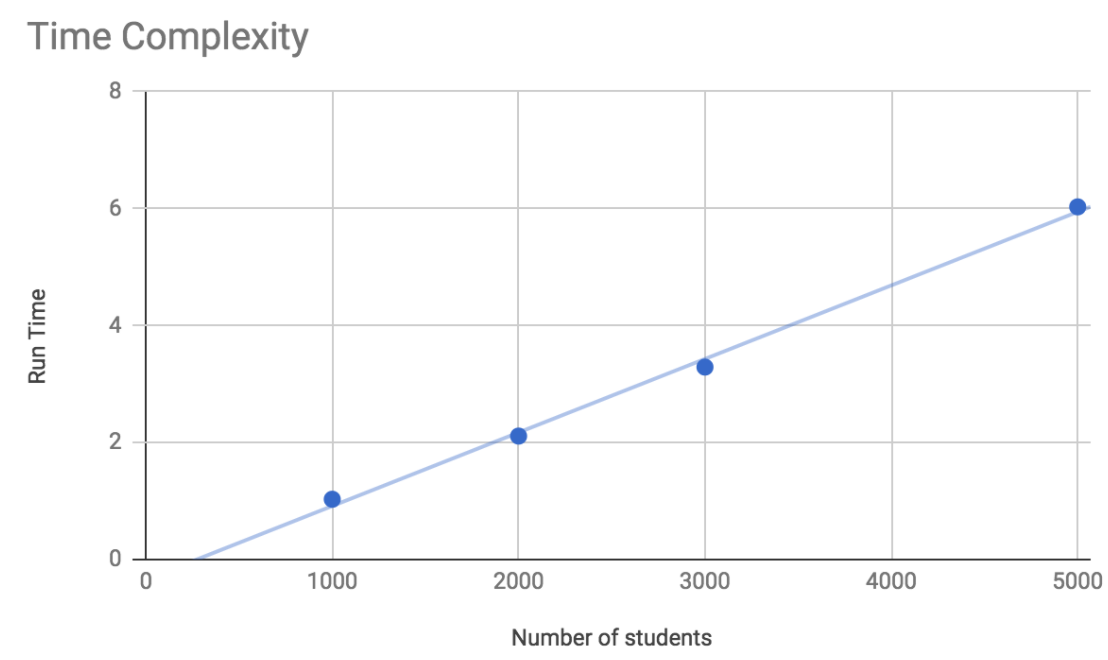
\includegraphics[scale =.6]{time-input}
 \caption{Average Time Taken: Basic}
 \label{timechart}
 \end{figure}\par
 \subsection{Quality Analysis}
\par We measure optimality of the result by \textit{student preference  value}, which is defined by the sum of the number of enrolled students in all classed, i.e. 
\[\text{student preferences value} = \sum_{c\in C} (\text{\# of students enrolled in }c)\]
\par Within each set of input, our algorithm shows a stable performance. For instance, for 3000 students, 8 times slots, 20 rooms, 160 classes (because the input generator only allows $c\leq rt$). On average, there are about $20$ classes assigned in the same time slots. So class time conflicts do exist. The standard deviation on \textit{student preferences value} is 95.5, with an average of 9623 total enrollment. Furthermore, the most significant stand deviation occurs when there're 5000 students, which we think is caused by the increasing occurrence of conflicts in students' schedule. 
\par Then consider the performance on $student$ $preferences$ $value$ for sets of input where number of rooms, classes time slots fixed and student size is the variable. We choose the lower bound of $student$ $preferences$ $value$ for each set of input. First, consider there're 10 time slots, 50 rooms, 360 classes. For this set of input, our student size ranges from 1000 to 5000. Computing $\frac{\text{student preferences value}}{\text{best case preferences value}}$, we find that for different size of students, the ratio is almost the same, with a standard deviation of 0.0009. Thus, the average of these ratios can represent the performance of our algorithm on these set of input. With an average of $0.86308125$, our algorithm can arrange $86\%$ of students for their preferred classes.\\ \\Then we repeat the experiment on different sets of input with 8 time slots, 20 rooms, 160 classes, and again student size ranges from 1000 to 5000, but this time with more realistic parameters. For these set of data, we apply the same analysis strategy and get an average of $0.8023$ ratio. This ratio means that for 8 time slots, 20 rooms, 160 classes, we can arrange $80\%$ of students for their preferred classes.\par
We think the difference between the two different ratios result from different number of time slots, and rooms. For the first set of data, there're 10 time slots, and 50 rooms, indicating more slots for classes and also a less occurrence of time conflicts. Under such a circumstance, our algorithm can arrange more classes and will thus generate a better performance.

\subsection{ Haverford Extension}
%==================Figure 2===================
\begin{figure}[H]
\centering
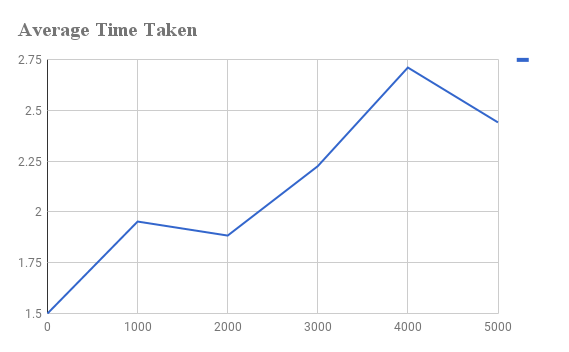
\includegraphics[scale =.6]{chart}
\caption{Average Time Taken: Haverford Extension}
\label{timechart-2}
\end{figure}
%=================Time Analysis=============
From Figure \ref{timechart-2}. we can see that even we have no student, we still need to do all these preparations in 1.5 seconds. Observe that the complexity is still near-linear, although the deviations are larger. The reason that it vibrates when the size of input increases is that the time spent on assigning student depends on the quality of random generated input. If the input has a lot of conflicts, we need to check time conflict much more than a good quality input file. Here, the overall quality of input with size 5000 is slightly better than expected. 

%==================Figure 1===================
\begin{figure}[H]
\centering
\begin{tabular}{ |c||c|c|c|c|c|c| } 
 \hline
 Number of students & $1000$  & $2000$ & $3000$ & $4000$ & $5000$\\ 
  \hline \hline 
 Optimal Student Preferences Value & $3131$ & $6136$  & $8485$ & $9489$ & $10365$ \\
  \hline
Worst Case Student Preferences Value& $1166$ & $2476$ & $6931$ & $8036$ & $5107$ \\ 
 \hline
Ave. Student Preferences Value& $2465.9$ & $5461$ & $7992$ & $8603$ & $8951$ \\
 \hline
 Ave. Time Taken & $1.9531$ & $1.88398$ & $2.2616$ & $2.71231$ & $2.44185$ \\
 \hline
\end{tabular}
\caption{Performance table}
\end{figure}
%=======quality analysis
Comparing to the performance shown in basic version, the Haverford extension version shows more variation. In this case, we only consider the number of rooms, classes time slots as fixed and vary student size only, because the time slots and classrooms will be imported from $HaverfordEnrollmentData$ file. We choose the lower bound of $student$ $preferences$ $value$ for each set of input. There are 58 time slots (many of them overlap with each other), 47 rooms, 268 classes, and we vary the student size from 1000 to 5000. The preference lists of students are generated by a new random input generator and the number of class each student wants to take varies between 2 - 7, considering student might want to take class in Bryn Mawr or Swarthmore. Computing $\frac{\text{student preferences value}}{\text{best case student value}}$, we find that for different size of students, the ratio decreases after the size of students reaches 3000. We found that when student size is 1000 - 3000, the performances of these three tests are $0.8219666667$ (size 1000), $0.9101666667$ (size 2000) and $0.888$ (size 3000), which means that our algorithm can arrange $82\%$ of students for their preferred classes, if there are 1000 students, and can arrange $91\%$ of students for their preferred class, when there are 2000 students. However, when the size of the student body is larger than $3000$, the total number of students enrolled in classes tends to vary a lot, depending on the input. So the performance here is $0.7222$ (4000) and $0.5967333333$ (5000) and we can see a obvious compromise of performance after 3000 students.
\\We think the possible reason of this compromise of performance is that the fixed available time slots and classrooms, especially the classrooms, limit the performance of our algorithm when we apply it on large size input. We checked the total capacity of all rooms in Haverford is 1153, with average capacity of 24 people per rooms, and for 5000 students, the reasonable conjecture of total population of all classes is 15000, which requires a lot of valid time slots to fit in. When there is not enough spot to assign classes, our algorithm will terminate and return the schedule. Hence, we believe our algorithm's performance will be much better if the we can have more classrooms with larger capacity. 
\\We also test our algorithm by the original student preference list parsed from 2014 HaverfordEnrollmentData. There are 1177 students and the performance of this test is $81\%$, it is similar to our result in testing 1000 students. 

\section{Recommendation and Improvement}
Based on our design process and experimental analysis, we have three recommendations to current registration office. Firstly, it would be better if registration office is able to get the popularity of each department and make schedule based on the popularity of department. For example Computer Science are highly demanded each semester. Therefore, making sure that these classes are offered in big classrooms is very important. Otherwise, student might not be able to get in those classes. Secondly, it is necessary to consider core courses list from each department, because these are classes students must take to fulfill they graduation requirement. Hence, we want to schedule these important and popular classes first into big classrooms. 
\par In our implementation, we still have several thoughts to improve our current scheduling algorithm but because of the approaching due date, we are not able to implement them but we would like to share our thoughts here. The first improvement is to add multiple lab sessions when we assign lab session. In our current implementation, we can only assign one lab for each course which requires lab, but some departments, say, chemistry and biology, may require more than one lab sessions. It will be better to consider this situation. The second improvement is to have a more selective check-time-conflict function. In our current implementation, we only check whether two class times conflict with each other, instead of knowing which class conflict with which. It will be better to get this information because we can assign scientific classes at the same time as the time assigned to social science or humanity classes, as students take them should be fairly different, especially in high level classes. So it is possible for student to have less conflicts in his class list if we do so. 
\end{document}

